%--------------------INTRODUCTION--------------------------------------
%This is the format for IISER Bhopal PhD Thesis for Physics or Mathematics.
%A modified version of the one originally prepared by Arghya Chattopadhyay (arghya.chattopadhyay@gmail.com). Huge shout out to Arghya for all the hard work!

%Be prepared to modify a bit the IISERB class file to conform with whoever incharge at the academic office PhD section. 

%The formatting related contents (packages, custom layout, fonts, etc.) are now part of the IISERB.cls class file, which also contains the title page layout. 
%All you have to do is enter your details in the individual details section below. 

%This version: 1.0.1 
%Created by: Sandeep Aashish
%contact: sandeepaashish@hotmail.com
%Date created: January 23, 2020

%--------------------INSTRUCTIONS---------------------------------
%COMPATIBILITY: pdflatex; bibtex; makeindex (for indexing and nomenclature with nomencl package)

%thesis.tex is the mainfile. Other included files (in folders: chapters, frontmatter, endmatter,commands) have a header: %!TEX root=../thesis.tex .
%Most of the required .sty files are in styles folder. Add them to your local latex installation folder (if you don't know how, google it!). 
%bibliography style file hunsrt.bst is also in the styles folder.

%On the first run, follow these steps:
%pdflatex > makeindex thesis.nlo -s nomencl.ist -o thesis.nls > bibtex > pdflatex (x2)

%You can add these arguments for makeindex in your editor's options menu.
%=====================================================================================

\documentclass{IISERB}

\makenomenclature
%For index generation.
%\makeindex 

%====================Set Graphics path============================

\graphicspath{{figures/}}


%=====================Command Modification=========================

%Either enter your modifications here or write them in a seperate file and include it here.

%!TEX root = ../thesis.tex

% Custom commands file. \include in mainfile

%=====================Command Modification=========================

%Either enter your modifications here or write them in a seperate file and include it here. Examples are written below


%%%%%%%%%%%%%%%% AMS THEOREM %%%%%%%%%%%%%%%%%%%%%%%%
\newtheorem{theorem}[equation]{Theorem}
\newtheorem*{theorem*}{Theorem}
\newtheorem{lemma}[equation]{Lemma}
\newtheorem*{lemma*}{Lemma}
\newtheorem{proposition}[equation]{Proposition}
\newtheorem*{proposition*}{Proposition}
\newtheorem{propdef}[equation]{Proposition and Definition}
\newtheorem{corollary}[equation]{Corollary}
\newtheorem*{corollary*}{Corollary}
\newtheorem{question}[equation]{Question}

\theoremstyle{definition}
\newtheorem{definition}[equation]{Definition}
\newtheorem*{definition*}{Definition}
\newtheorem{notation}[equation]{Notation}
\newtheorem{observation}[equation]{Observation}
\newtheorem{claim}[equation]{Claim}

\theoremstyle{remark}
\newtheorem{remark}[equation]{Remark}
\newtheorem{remarks}[equation]{Remarks}
\newtheorem{example}[equation]{Example}
%%%%%%%%%%%%%%%%%%%%%%%

\newcommand{\N}{\mathbb{N}}
\newcommand{\Z}{\mathbb{Z}}
\newcommand{\Q}{\mathbb{Q}}
\newcommand{\R}{\mathbb{R}}
\newcommand{\C}{\mathbb{C}}

% ===============================================================


\DeclarePairedDelimiter{\abs}{\lvert}{\rvert}% absolute value
\DeclarePairedDelimiter{\norm}{\lVert}{\rVert}% norm
\DeclarePairedDelimiter{\ket}{\lvert}{\rangle}% ket-bra notation
\DeclarePairedDelimiter{\bra}{\langle}{\rvert}% ket-bra notation
\DeclarePairedDelimiterX{\braket}[2]{\langle}{\rangle}{#1\,\delimsize\vert\,\mathopen{}#2}% inner product
\DeclarePairedDelimiterX{\inpro}[2]{\langle}{\rangle}{#1, #2}% inner product
\DeclarePairedDelimiterX{\setgiven}[2]{\{}{\}}{#1\,{:}\,\mathopen{}#2}% set given by



%=====================For Dummyx text, tables and figures===============
%One can comment this section out

%\usepackage{lipsum}
%\usepackage{sator}

%===============================================================



% ------------------------------
% Individual details (Change these!)
% ------------------------------

% don't forget to remove the square brackets

\newcommand{\thesistitle}{[Thesis Title]}%Include your thesis title
\newcommand{\studentname}{[Student Name]}%Change it to your name
\newcommand{\salutation}{[Mr./Ms.]}% Mr. or Ms. or anything
\newcommand{\studentrollno}{[Roll Number]}%Change it to your roll number
\newcommand{\advisorname}{[Supervisor]}%Change it to your advisor's name
\newcommand{\subject}{[Department]}%Change it to physics or maths
\newcommand{\thesisdate}{[Month, year]}%Include thesis year
\newcommand{\vivadate}{[Month, year]}%Include viva date, keep it same as the thesis date while forwarding for evaluation
\newcommand{\thesisyear}{[year]}%Again input the year for convinience
\newcommand{\external}{[name of Ex. Examiner]}%Input the name of external examiner
\newcommand{\memberone}{[name of the oral board examiner]}%Input the name of the member
\newcommand{\membertwo}{[name of the oral board examiner]}%Input the name of the member
\newcommand{\memberthre}{[name of the oral board examiner]]}%Input the name of the member




\begin{document}

\frontmatter

\begin{titlepage}
\maketitle
\end{titlepage}
%%%%%%%%%%%%% 2nd title %%%%%%%%%%%%%
\newpage

\begin{titlepage}
\maketitle
\end{titlepage}



\pagebreak

%!TEX root=../thesis.tex

%\vspace{2cm}
\begin{center}\Large{\textbf{CERTIFICATE}}\end{center}
\vspace{0.5cm}

{\fontfamily{ppl}\selectfont
	\noindent The undersigned have examined the Ph.D. thesis entitled:}
\vspace{0.5cm}
\begin{center}\textbf{\thesistitle}\end{center}
\vspace{0.5cm}
{\fontfamily{ppl}\selectfont
	presented by  \studentname, a candidate for the degree of \mbox{Doctor of Philosophy} in the department of \subject, and hereby certify that it is worthy of acceptance.
	
	\vspace{1.3cm}
	\parbox{0.6\textwidth}{ 
		\flushleft{[Date]}
		\vspace{16cm}
	}
	\hfill 
	\parbox{0.4\textwidth}{
		\mbox{[Signature]} \\
		\mbox{[Name of the oral board examiner]}\\
		External Examiner\\
		
		\vspace{1.3cm}
		\mbox{[Signature]}\\
		\mbox{[Name of the oral board examiner]}\\
		Supervisor\\
		
		\vspace{1.3cm}
		\mbox{[Signature]}\\
		\mbox{[Name of the oral board examiner]}\\
		Member\\
		
		\vspace{1.3cm}
		\mbox{[Signature]}\\
		\mbox{[Name of the oral board examiner]}\\
		Member\\
		
		\vspace{1.3cm}
		\mbox{[Signature]}\\
		\mbox{[Name of the oral board examiner]}\\
		Member\\
	}
}
\addcontentsline{toc}{chapter}{Certificate}
\newpage

\addcontentsline{toc}{chapter}{Academic Integrity and Copyright Disclaimer}
%!TEX root=../thesis.tex


%\hspace{2cm}
\begin{center}
	\Large{\textbf{ACADEMIC INTEGRITY AND COPYRIGHT \\
			\vspace{0.5cm}
			DISCLAIMER}}
\end{center}
{\fontfamily{ppl}\selectfont
	I hereby declare that this thesis is my own work and, to the best of
	my knowledge, it contains no materials previously published or written
	by any other person, or substantial proportions of material which have
	been accepted for the award of any other degree or diploma at IISER
	Bhopal or any other educational institution, except where due
	acknowledgement is made in the thesis.
	
	
	\noindent I certify that all copyrighted material incorporated into this thesis is in compliance with the Indian Copyright (Amendment) Act, 2012 and that I have received written permission from the copyright owners for my use of their work, which is beyond the scope of the law. I agree to indemnify and save harmless IISER Bhopal from any and all claims that may be asserted or that may arise from any copyright violation.
	
	\vspace{4cm}
	\parbox{0.7\textwidth}{ 
		\flushleft{\thesisdate\\IISER Bhopal}
	}
	\hfill 
	\parbox{0.3\textwidth}{ 
		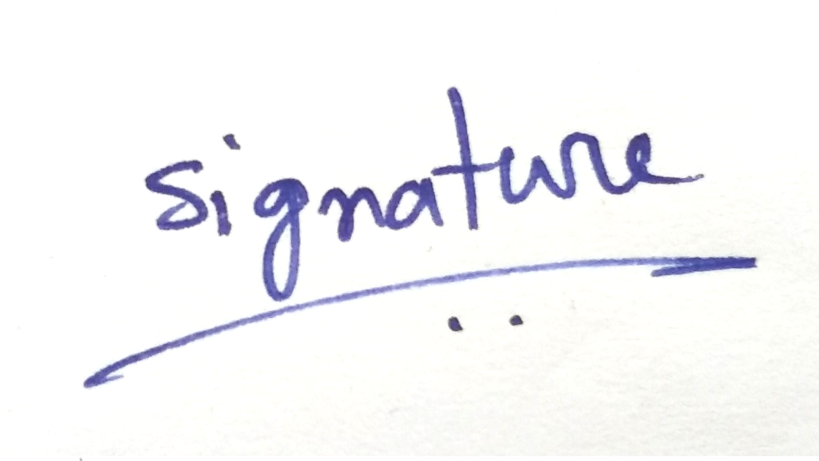
\includegraphics[width=4cm]{sign}
		\mbox{\studentname}
	}
}
\newpage

\addcontentsline{toc}{chapter}{Acknowledgement}
%!TEX root=../thesis.tex


\begin{center}
{\textbf{\Large{Acknowledgements}}}
 \end{center}
 Put the acknowledgement
\newpage

\addcontentsline{toc}{chapter}{Dedication}
%!TEX root=../thesis.tex


\begin{center}\Large{\textbf{DEDICATION}}\end{center}

(Optional) Dedicated to the dedicated
\newpage

\addcontentsline{toc}{chapter}{Abstract}
%!TEX root=../thesis.tex

\begin{center}\Large{\textbf{ABSTRACT}}\end{center}
Abstract




\let\thefootnote\relax\footnote{\emph{Keywords}: (write the keywords
  for the research document) groupoid; C*-algebra; representation;
  topological correspondence; Fell bundle}
\let\thefootnote\relax\footnote{\emph{Subjclass[2010]}: (choose the
  subject class classification as per you choice and replace 2010 by
  it. Then replace the subject codes.) 46L55, 22A22}
\newpage

\addcontentsline{toc}{chapter}{Table of Contents}
\tableofcontents

\pagestyle{fancy}
\clearpage

\pagenumbering{arabic}


\mainmatter
%=====================Chapters==============================================
\newpage


%!TEX root = ../thesis.tex

\chapter{The title of chapter one}


\section{Quick examples}

Example of citation~\cite{dummy-1} and~\cite{dummy-2}.


Write \(\N,\Z,\Q,\R,\C\).

\(\norm{a}, \abs{b}, \ket{c}, \bra{d}, \braket{e}{f}, \inpro{g}{h}, \nicefrac{3}{\pi}\)

\begin{theorem}
  \label{thm:dummy-thm}
  A
\end{theorem}

\begin{theorem*}[Theorem of second dummy]
  A, follows from Theorem~\ref{thm:dummy-thm}
\end{theorem*}

\begin{lemma}
  \label{lem:dummy}
  Statement
\end{lemma}


\begin{example}
  \label{exa:haha}
  Null example.
\end{example}

\begin{equation}
  \label{eq:nontrivial}
  x^2=x^2.
\end{equation}
Note that Equation~\eqref{eq:nontrivial} is not an obvious fact. You need to scratch your head for it.

\begin{definition}
  \label{def:empty}
  This defintion is not empty.
\end{definition}
\begin{remark}
  \label{rem:regarding-def}
  The reader may find Definition~\ref{def:empty} nonempty, however, you can prove that the definition \emph{is} empty.
\end{remark}

List of environments can be found in the .cls file.



Commutative diagramme using tikz-cd.

\[
  \begin{tikzcd}
  T
\arrow[drr, bend left, "x"]
\arrow[ddr, bend right, "y"]
\arrow[dr, dotted, "{(x,y)}" description] & & \\
& X \times_Z Y \arrow[r, "p"] \arrow[d, "q"] & X \arrow[d, "f"] \\
& Y \arrow[r, "g"] &Z
\end{tikzcd}
\]


Example of commutative diagramme using TikZ.
    \begin{center}
      \begin{tikzpicture}[scale=1]
        \draw[->] (1.7,0)--(5.2,0); \draw[->] (0,1.7)--(0,0.2);
        \draw[->](2.5,2)--(4.4,2); \draw[->] (5.8, 1.7)--(5.8,0.24);
        \draw[->, double] (1.8, 0.6)--(4.2,1.4); \node at (6, 0)[
        scale=1]{$\mathfrak{S}(A,D)$}; \node at (6.2, 2)[
        scale=1]{$\mathfrak{S}(A,B)\times \mathfrak{S}(B,D)$}; \node
        at (-0.2, 2)[
        scale=1]{$\mathfrak{S}(A,B)\times \mathfrak{S}(B,C)\times
          \mathfrak{S}(C,D)$}; \node at (2.7,1.1)[scale=0.8]{$\sim$};
        \node at (3.8,0.8)[scale=0.8]{$a(A,B,C,D)$}; \node at (0, 0)[
        scale=1]{$\mathfrak{S}(A,C)\times \mathfrak{S}(C,D)$}; \node
        at (3.45, 2.25)[scale=0.8]{$\textup{Id}\times c(B,C,D)$};
        \node at (-1.1,
        1.0)[scale=0.8]{$ c(A,B,C)\times \textup{Id}$}; \node at (3.1,
        -0.2)[scale=0.8]{$c(A,C,D)$}; \node at (6.6,
        1.0)[scale=0.8]{$c(A,B,D)$};
      \end{tikzpicture}
    \end{center}

    Commutative diagramme using package XY.
    
    \begin{figure}[htb]
      \[
        \xymatrix@1@C=3em{ (G,\alpha)\quad
      \ar@/^1pc/[r]^{(X,\lambda)}_{}="0"
      \ar@/_1pc/[r]_{(Y,\kappa)}^{}="1" \ar@{=>}"0";"1"^{\phi} &
      \quad(H,\beta)\quad \ar@/^1pc/[r]^{(X',\lambda')}_{}="0"
      \ar@/_1pc/[r]_{(Y',\kappa')}^{}="1" \ar@{=>}"0";"1"^{\phi'}&
      \quad(K,\mu) }
  \]
    \caption{}
    \label{fig:vert-comp}
  \end{figure}


  Refer the packages for details about commutative diagrammes (type
  \verb+ texdoc tikz-cd+ or
  \verb+ texdoc xy+ and enter, or ask the internet).


 Glossaries ---regular glossaries, or glossaries appearing as list of
 symbols, etc--- are supported with package \emph{glossaries}. It can
 be used in the standard way. The package does not have \emph{xindy} option.

 Package \emph{xcolor} is loaded with \emph{x11names} option.

 Avoid working out~\ref{rem:more-details} and~\ref{rem:renaming-env}
 unless you know what you are doing.
 \begin{remark}
   \label{rem:more-details}
   Please have a look at \emph{commands.tex} and \emph{symbols.tex},
   in commands folder, for various shortforms and newcommands. You may
   modify and add new newcommands here. The packages are listed in
   IISERB.cls. You may add or modify the packages as per your need.
 \end{remark}
  
  \begin{remark}
    \label{rem:renaming-env}
    If you want, you may modify the math-theorem commands to use
    \verb+ \begin{thm}+ instead of
    \verb+ \begin{theorem}+ , and similar
    for other environments like proposition, examples, remarks. Check
    out the \emph{command.tex} in the commands folder.
  \end{remark}
  
\section{Dummy text}

In mathematics, a group is a set equipped with a binary operation that combines any two elements to form a third element in such a way that four conditions called group axioms are satisfied, namely closure, associativity, identity and invertibility. One of the most familiar examples of a group is the set of integers together with the addition operation, but groups are encountered in numerous areas within and outside mathematics, and help focusing on essential structural aspects, by detaching them from the concrete nature of the subject of the study.

\section{Philosophical discussion about groups}
\label{sec:grp-philo}

Groups share a fundamental kinship with the notion of symmetry. For example, a symmetry group encodes symmetry features of a geometrical object: the group consists of the set of transformations that leave the object unchanged and the operation of combining two such transformations by performing one after the other. Lie groups are the symmetry groups used in the Standard Model of particle physics; Poincaré groups, which are also Lie groups, can express the physical symmetry underlying special relativity; and point groups are used to help understand symmetry phenomena in molecular chemistry.

\subsection{More philosophy!}
\label{subsec:grp-philo}

The concept of a group arose from the study of polynomial equations, starting with Évariste Galois in the 1830s, who introduced the term of group (groupe, in French) for the symmetry group of the roots of an equation, now called a Galois group. After contributions from other fields such as number theory and geometry, the group notion was generalized and firmly established around 1870. Modern group theory—an active mathematical discipline—studies groups in their own right. To explore groups, mathematicians have devised various notions to break groups into smaller, better-understandable pieces, such as subgroups, quotient groups and simple groups. In addition to their abstract properties, group theorists also study the different ways in which a group can be expressed concretely, both from a point of view of representation theory (that is, through the representations of the group) and of computational group theory. A theory has been developed for finite groups, which culminated with the classification of finite simple groups, completed in 2004.Since the mid-1980s, geometric group theory, which studies finitely generated groups as geometric objects, has become an active area in group theory.

\section{A random jump to Hilbert spaces}

\textbf{This jump is because we wish to show you the header of a non-chapter right page.}

The mathematical concept of a Hilbert space, named after David Hilbert, generalizes the notion of Euclidean space. It extends the methods of vector algebra and calculus from the two-dimensional Euclidean plane and three-dimensional space to spaces with any finite or infinite number of dimensions. A Hilbert space is an abstract vector space possessing the structure of an inner product that allows length and angle to be measured. Furthermore, Hilbert spaces are complete: there are enough limits in the space to allow the techniques of calculus to be used.

Hilbert spaces arise naturally and frequently in mathematics and physics, typically as infinite-dimensional function spaces. The earliest Hilbert spaces were studied from this point of view in the first decade of the 20th century by David Hilbert, Erhard Schmidt, and Frigyes Riesz. They are indispensable tools in the theories of partial differential equations, quantum mechanics, Fourier analysis (which includes applications to signal processing and heat transfer), and ergodic theory (which forms the mathematical underpinning of thermodynamics). John von Neumann coined the term Hilbert space for the abstract concept that underlies many of these diverse applications. The success of Hilbert space methods ushered in a very fruitful era for functional analysis. Apart from the classical Euclidean spaces, examples of Hilbert spaces include spaces of square-integrable functions, spaces of sequences, Sobolev spaces consisting of generalized functions, and Hardy spaces of holomorphic functions.

Geometric intuition plays an important role in many aspects of Hilbert space theory. Exact analogs of the Pythagorean theorem and parallelogram law hold in a Hilbert space. At a deeper level, perpendicular projection onto a subspace (the analog of "dropping the altitude" of a triangle) plays a significant role in optimization problems and other aspects of the theory. An element of a Hilbert space can be uniquely specified by its coordinates with respect to a set of coordinate axes (an orthonormal basis), in analogy with Cartesian coordinates in the plane. When that set of axes is countably infinite, the Hilbert space can also be usefully thought of in terms of the space of infinite sequences that are square-summable. The latter space is often in the older literature referred to as the Hilbert space. Linear operators on a Hilbert space are likewise fairly concrete objects: in good cases, they are simply transformations that stretch the space by different factors in mutually perpendicular directions in a sense that is made precise by the study of their spectrum.

% \begin{theorem}
%   This is theorem.
% \end{theorem}




%!TEX root = ../thesis.tex

\chapter{The title of chapter two}


The integers, along with the two operations of addition and
multiplication, form the prototypical example of a ring.  In
mathematics, a ring is one of the fundamental algebraic structures
used in abstract algebra. It consists of a set equipped with two
binary operations that generalize the arithmetic operations of
addition and multiplication. Through this generalization, theorems
from arithmetic are extended to non-numerical objects such as
polynomials, series, matrices and functions.

A ring is an abelian group with a second binary operation that is
associative, is distributive over the abelian group operation, and has
an identity element (this last property is not required by some
authors, see § Notes on the definition). By extension from the
integers, the abelian group operation is called addition and the
second binary operation is called multiplication.

Whether a ring is commutative or not (that is, whether the order in which two elements are multiplied changes the result or not) has profound implications on its behavior as an abstract object. As a result, commutative ring theory, commonly known as commutative algebra, is a key topic in ring theory. Its development has been greatly influenced by problems and ideas occurring naturally in algebraic number theory and algebraic geometry. Examples of commutative rings include the set of integers equipped with the addition and multiplication operations, the set of polynomials equipped with their addition and multiplication, the coordinate ring of an affine algebraic variety, and the ring of integers of a number field. Examples of noncommutative rings include the ring of \(n \times n\) real square matrices with \(n \geq 2\), group rings in representation theory, operator algebras in functional analysis, rings of differential operators in the theory of differential operators, and the cohomology ring of a topological space in topology.



%!TEX root = ../thesis.tex

\chapter{Third chapter}

In mathematics, a field is a set on which addition, subtraction, multiplication, and division are defined and behave as the corresponding operations on rational and real numbers do. A field is thus a fundamental algebraic structure which is widely used in algebra, number theory, and many other areas of mathematics.

The best known fields are the field of rational numbers, the field of real numbers and the field of complex numbers. Many other fields, such as fields of rational functions, algebraic function fields, algebraic number fields, and p-adic fields are commonly used and studied in mathematics, particularly in number theory and algebraic geometry. Most cryptographic protocols rely on finite fields, i.e., fields with finitely many elements.

The relation of two fields is expressed by the notion of a field extension. Galois theory, initiated by Évariste Galois in the 1830s, is devoted to understanding the symmetries of field extensions. Among other results, this theory shows that angle trisection and squaring the circle cannot be done with a compass and straightedge. Moreover, it shows that quintic equations are algebraically unsolvable.

Fields serve as foundational notions in several mathematical domains. This includes different branches of mathematical analysis, which are based on fields with additional structure. Basic theorems in analysis hinge on the structural properties of the field of real numbers. Most importantly for algebraic purposes, any field may be used as the scalars for a vector space, which is the standard general context for linear algebra. Number fields, the siblings of the field of rational numbers, are studied in depth in number theory. Function fields can help describe properties of geometric objects.



\include{chapters/conclusion}


\backmatter

%==============================Appendices===================================
\appendix
\appendixpage
%\suppresschapternumber
%\removedotbetweenchapterandsection


%!TEX root = ../thesis.tex

\chapter{Appendix A: Division ring}
\label{AppendixA}

Dropping one or several axioms in the definition of a field leads to other algebraic structures. As was mentioned above, commutative rings satisfy all axioms of fields, except for multiplicative inverses. Dropping instead the condition that multiplication is commutative leads to the concept of a division ring or skew field.[nb 7] The only division rings that are finite-dimensional \(R\)-vector spaces are \(R\) itself, \(\C\) (which is a field), the quaternions \(\mathbb{H}\) (in which multiplication is non-commutative), and the octonions \(\mathbb{O}\) (in which multiplication is neither commutative nor associative). This fact was proved using methods of algebraic topology in 1958 by Michel Kervaire, Raoul Bott, and John Milnor. The non-existence of an odd-dimensional division algebra is more classical. It can be deduced from the hairy ball theorem illustrated at the right.
%========To generate dummy table, delete to write new===============
%\satortab
%=========================================================
%\chapter{Second Appendix}
%========To generate dummy figure, delete to write new===============
%\satorfig
%=========================================================


% =============================Bibliography=====================================
\singlespacing
\addcontentsline{toc}{chapter}{References}
\bibliographystyle{plain}   %bibliography style
\renewcommand{\bibname}{References} %bibliography chapter header
\bibliography{endmatter/mybib} %.bib file source


%=============Generating List of figures and list of tables================

\addcontentsline{toc}{chapter}{List of Figures}
\listoffigures

(Optional for mathematics)


\addcontentsline{toc}{chapter}{List of Tables}
\listoftables

(Optional for mathematics)

%====================Symbols================================

\chapter{List of Symbols}
% \addcontentsline{toc}{chapter}{List of Symbols}%

Optional

%!TEX root = ../thesis.tex
%Add your own list of symbols

%====================Symbols================================
%Below is the example to add list of symbols. You can add them in the main text as well in this same format.

%\begin{center}\Large{\textbf{List of Symbols}}\end{center}


\nomenclature{$\mathbb{B}(H,K)$}{Set of bounded operators from \(H\)
  to \(K\)} 
\nomenclature{$\mathbb{K}$}{Compact operators on \(\ell^2\)} 
\nomenclature{$\mathcal$(H)}{Compact operators on \(H\)} 
\nomenclature{$\mathcal{F}$}{The Fourier transform} 

\printnomenclature

%============================================================




%!TEX root=../thesis.tex


\thispagestyle{empty}
\rotatebox[origin=c]{270}{Ph.D. Thesis}

\vspace{7cm}

\rotatebox[origin=c]{270}{\mbox{\studentname}}

\vspace{7cm}

\rotatebox[origin=c]{270}{\thesisyear}

\end{document}
